% !TEX TS-program = pdflatexmk
%% ---------------------------------------------------
%% -- Stand: 2024/03/10
%% -- Datei für die Erstellung des Beitrags 
%% -- Wir nutzen KOMA-Script  
%% ---------------------------------------------------
\documentclass[%
	,ngerman					 
	,bibliography 	= leveldown  
%	,parskip = half+			 
	]{scrbook}


%% -- Hier finden sich die wesentlichen Definitionen
%% --
\usepackage{./preamble/Rom-Beitrag}	

%% -- Literaturverzeichnis
%% --
\addbibresource{./content-abcd/bib-abcd/Biblio-abcd.bib}	

%% -- Eigene, zusätzliche Definitionen
%% -- 
%% -----------------------------------------------------
%% -- Für die eigenen Definitionen
%% -- Stand: 2023/02/02
%% -- Wissen, was man macht ist notwendig
%% ----------------------------------------------------- 

%% -- Für was dokumentierens
%% -- 

%% -- Einstellungen Dictum; siehe KOMA Seite 138-140
%% --
\renewcommand{\dictumwidth}{0.45\textwidth}

%% -- Wir starten nun
%% --
\begin{document}

%% -- Der Beitrag in separater Datei
%% --
% !TEX root = ../Rom-abcd.tex
%% -----------------------------------------------------
%% -- Musterdatei für die Erstellung des Beitrags
%% -- Stand: 2023/02/08
%% -----------------------------------------------------
%% -- Definitionen, damit die Eingabe einfacher wird
%% -- Bitte \renewcommand belassen
%% --
\renewcommand{\LongTitel}{Langform des Titels}
\renewcommand{\ShortTitel}{Kurzform des Titel}
\renewcommand{\AutorenBeitrag}{Autor1, Autor2 \& Autor3}

%% -- Kapitelüberschrift und Eintrag in TOC
%% --
\addchap[\ShortTitel]{\LongTitel}
\addtocontents{toc}{\textsc{\AutorenBeitrag}}
\addtocontents{toc}{}

%% -- Kopfzeile 
%% -- Gerade Seiten : Autoren
%% -- Ungerade Seiten: Kurztitel
%% --
\markleft{\textsc{\AutorenBeitrag}}	
\markright{\textsc{\ShortTitel}}	

%% -- Titelseite des Beitrags inkl. Bild
%% -- des/der Vortragenden
%% --
\begin{center}
	\textsc{\Large \AutorenBeitrag}\\[1.5em]
	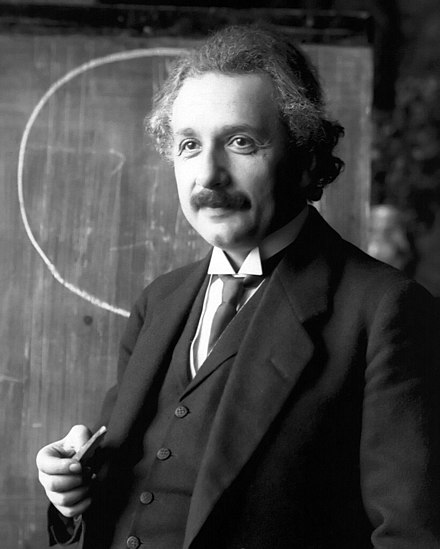
\includegraphics[width=8cm, height=8cm, keepaspectratio=true]{./content-abcd/autor1}
\end{center}

%% -- Wer einen sinnvollen Spruch nutzen will
%% -- dann bitte mit \dictum[]{}; Größe kann man anpassen
%% --
\renewcommand{\dictumwidth}{0.45\textwidth}
\dictum[\href{https://de.wikipedia.org/wiki/Albert_Einstein}{Albert Einstein}]{Wahnsinn ist, dasselbe immer  \mbox{wieder} zu tun und andere Ergebnisse zu erwarten.}
%%
\begin{quote}
Für eine kurze Zusammenfassung des Beitrags -- sollte schon sein.
\end{quote}

%% -- Referenzen des Beitrags am Ende
%% --
\begin{refsection}
%% --
\section*{Erster Hauptabschnitt}		%% 
\subsection*{Erster Unterabschnitt}		%% 
\blindtext	
%%				
\subsection*{Zweiter Unterabschnitt}
\blindtext	
%% --
\section*{Zweiter Hauptabschnitt}		%% 
\subsection*{Erster Unterabschnitt}		%% 
\blindtext	
%% -- etc.
%% --

%% -- Literaturverzeichnis
%% --
\RaggedRight
\nocite{*}
\printbibliography
\end{refsection}



%% --
\end{document} 